\chapter{Space-Filling Curves}
\label{ch:space_filling_curves}

\section{Hilbert Curve}
\label{sec:hilbert_curve}

\subsection{Overview}
The \index{Hilbert curve}Hilbert curve is a continuous fractal \index{space-filling curve}space-filling curve first described by David Hilbert in 1891~\cite{hilbert1891}. It is a mapping between 1D and 2D (or higher-dimensional) space that preserves \index{locality preservation}locality: points that are close together on the 1D curve are also close together in the 2D plane. This property makes the Hilbert curve an invaluable tool for multidimensional indexing, data compression, and spatial analysis~\cite{sagan1994}.

\subsection{Definitions}
\begin{definition}[Space-Filling Curve]\label{def:space_filling_curve}
A continuous function $f \colon [0,1] \to [0,1]^2$ whose range contains the entire 2-dimensional unit square. Formally, $f$ is \emph{surjective}: for every point $(x, y) \in [0,1]^2$, there exists $t \in [0,1]$ such that $f(t) = (x, y)$~\cite{sagan1994}.
\end{definition}

\begin{definition}[Order ($n$)]\label{def:hilbert_order}
The number of recursive subdivisions. An order-$n$ Hilbert curve covers a grid of $2^n \times 2^n$ cells and visits all $4^n$ cells exactly once. The total curve length at order $n$ is $2^n - 1$ cell-to-cell transitions.
\end{definition}

\begin{definition}[Locality Preservation]\label{def:locality_preservation}
The property where distance on the curve (Hilbert index) correlates strongly with Euclidean distance in space. Specifically, for points $p, q \in [0,1]^2$ with Hilbert indices $h(p), h(q)$, the Hilbert distance $|h(p) - h(q)|$ is bounded by a polynomial function of the Euclidean distance $\|p - q\|$~\cite{moon2001}.
\end{definition}

\begin{definition}[U-shape]\label{def:u_shape}
The basic motif of the Hilbert curve, which is rotated and reflected to form higher orders. The four orientations of the U-shape determine how the sub-curves connect at each level of recursion.
\end{definition}

\subsection{Theory}
The Hilbert curve is constructed recursively. For order $n=1$, it is a simple U-shape connecting four cells. To create order $n+1$:
\begin{enumerate}
    \item The space is divided into four quadrants.
    \item Four order-$n$ curves are placed in the quadrants.
    \item The bottom-left curve is rotated $90^\circ$ clockwise.
    \item The bottom-right curve is rotated $90^\circ$ counter-clockwise and reflected.
    \item The four curves are connected by three segments.
\end{enumerate}

The transformation from 2D coordinates $(x, y)$ to a 1D index $d$ (and vice versa) involves bitwise operations and coordinate rotations. As the order $n \to \infty$, the curve fills the entire square.

\begin{theorem}[Locality Bound of the Hilbert Curve]\label{thm:hilbert_locality}
For any two points $p, q \in [0,1]^2$ with Hilbert indices $h(p)$ and $h(q)$, there exists a constant $c > 0$ such that:
\[
|h(p) - h(q)| \le c \cdot \|p - q\|_1 \cdot \max\!\left(\frac{1}{\|p - q\|_1}, 1\right)^{\log_2 d},
\]
where $d$ is the dimension. In 2D, this simplifies to the bound that points within a Hilbert-index window of width $w$ are contained in a square of side length $O(\sqrt{w})$~\cite{moon2001}.
\end{theorem}

\begin{proof}
The proof follows from the self-similar structure of the Hilbert curve. At each level $k$ of the recursion, the space is partitioned into $4^k$ cells, each of side length $2^{-k}$. Two points in the same level-$k$ cell have Hilbert indices differing by at most $4^k$. Conversely, if their Hilbert indices differ by $\Delta$, they must share a common ancestor cell at level $k = \lceil \log_4 \Delta \rceil$, which has side length $2^{-k} \le 2\sqrt{\Delta}$. This gives the $O(\sqrt{w})$ spatial bound for a window of width $w$~\cite{moon2001}.
\end{proof}

\begin{example}[Hilbert Curve of Order 2]\label{ex:hilbert_order2}
An order-2 Hilbert curve visits all $4^2 = 16$ cells in a $4 \times 4$ grid. Starting from the bottom-left corner $(0, 0)$:
\[
(0,0) \to (1,0) \to (1,1) \to (0,1) \to (0,2) \to (0,3) \to (1,3) \to (1,2) \to
\]
\[
(2,2) \to (2,3) \to (3,3) \to (3,2) \to (3,1) \to (2,1) \to (2,0) \to (3,0)
\]
Points that are consecutive on the curve are always Manhattan neighbors (differing in exactly one coordinate by 1). The four quadrants each contain an order-1 U-shape, rotated and reflected as prescribed by the recursive construction~\cite{sagan1994}.
\end{example}

\begin{figure}[htbp]
\centering
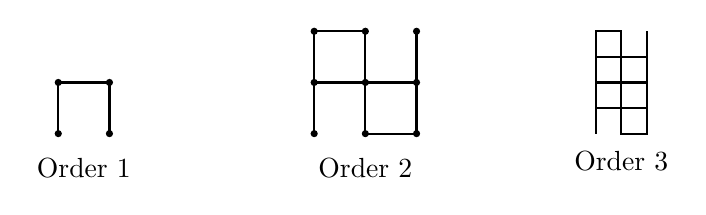
\begin{tikzpicture}[scale=0.65]
  \begin{scope}[xshift=-5cm]
    \draw[thick] (0,0)--(0,1)--(1,1)--(1,0);
    \foreach \x/\y in {0/0,0/1,1/1,1/0} {\fill (\x,\y) circle (2pt);}
    \node[below] at (0.5,-0.3) {Order 1};
  \end{scope}
  \begin{scope}[xshift=0cm]
    \draw[thick] (0,0)--(0,2)--(1,2)--(1,1)--(0,1)--(0,2) (1,1)--(2,1)--(2,2) (2,1)--(2,0)--(1,0)--(1,1);
    \foreach \x/\y in {0/0,0/1,0/2,1/2,1/1,2/1,2/2,2/0,1/0} {\fill (\x,\y) circle (2pt);}
    \node[below] at (1,-0.3) {Order 2};
  \end{scope}
  \begin{scope}[xshift=5.5cm,scale=0.5]
    \draw[thick] (0,0)--(0,4)--(1,4)--(1,3)--(0,3)--(0,4) (1,3)--(2,3)--(2,4) (2,3)--(2,2)--(1,2)--(1,3) (1,2)--(0,2)--(0,3) (0,2)--(0,1)--(1,1)--(1,2) (1,1)--(2,1)--(2,2) (2,1)--(2,0)--(1,0)--(1,1);
    \node[below] at (1,-0.3) {Order 3};
  \end{scope}
\end{tikzpicture}
\caption{Hilbert curve construction: each order recursively places four rotated copies in a U-shaped pattern.}
\label{fig:hilbert_curve}
\end{figure}


\subsection{Pseudocode}
\begin{algorithm}
\caption{Hilbert Curve: Coordinates to Index}\label{alg:xy_to_hilbert}
\begin{algorithmic}
\Function{XYtoHilbert}{n, x, y}
    \State $d \gets 0$
    \State $s \gets 2^{n - 1}$
    \While{$s > 0$}
        \State $rx \gets (x \ \& \ s) > 0$
        \State $ry \gets (y \ \& \ s) > 0$
        \State $d \gets d + s \cdot s \cdot ((3 \cdot rx) \oplus ry)$
        \Comment{Rotate and flip}
        \State $x, y \gets \text{RotateHilbert}(s, x, y, rx, ry)$
        \State $s \gets \lfloor s / 2 \rfloor$
    \EndWhile
    \Return $d$
\EndFunction

\Statex

\Function{RotateHilbert}{n, x, y, rx, ry}
    \If{$ry = 0$}
        \If{$rx = 1$}
            \State $x \gets n - 1 - x$
            \State $y \gets n - 1 - y$
        \EndIf
        \Return $y, x$
    \EndIf
    \Return $x, y$
\EndFunction
\end{algorithmic}
\end{algorithm}
\Cref{alg:xy_to_hilbert} converts 2D coordinates to a 1D Hilbert index using $O(n)$ bitwise operations. The inverse mapping \texttt{HilbertToXY} follows the same logic in reverse~\cite{hilbert1891,sagan1994}.

\subsection{Parameter Selection}
\begin{itemize}
    \item \textbf{Order ($n$)}: Typically chosen so that $2^n$ matches the resolution of the spatial grid.
    \item \textbf{Dimension}: While most common in 2D, the Hilbert curve can be extended to any number of dimensions $k$.
\end{itemize}

\subsection{Complexity}
\begin{itemize}
    \item \textbf{Transformation}: $O(n)$ bitwise operations for an order-$n$ curve. For a fixed grid size, this is essentially $O(1)$.
    \item \textbf{Space}: $O(1)$ auxiliary space to perform the coordinate mapping.
\end{itemize}

\subsection{Usages}
\begin{itemize}
    \item \textbf{Spatial Indexing}: Organizing data in databases (like MongoDB or GeoJSON) for faster range queries.
    \item \textbf{Image Dithering}: Ordering pixels for error diffusion to minimize visual artifacts.
    \item \textbf{Parallel Computing}: Mapping multidimensional tasks to linear processing units while maintaining local data relationships (e.g., in domain decomposition).
    \item \textbf{Data Compression}: Improving the performance of compression algorithms by clustering similar nearby values.
    \item \textbf{Cache Optimization}: Storing 2D arrays in Hilbert order to improve the L1/L2 cache hit rate for local access patterns.
\end{itemize}

\subsection{Testing Methods and Edge Cases}
\begin{itemize}
    \item \textbf{Invertibility}: Verify that \texttt{HilbertToXY(XYtoHilbert(x, y)) == (x, y)} for all points in a grid.
    \item \textbf{Adjacency}: Verify that points with sequential indices $d, d+1$ are always Manhattan neighbors in the 2D grid.
    \item \textbf{Large Order}: Test the transformation with $n=31$ to ensure bitwise operations don't overflow 64-bit integers.
    \item \textbf{All Quadrants}: Test points in each of the four main quadrants to ensure rotation and reflection logic is correct.
\end{itemize}

\subsection{References}
\begin{itemize}
    \item Hilbert, D. (1891). ``\"Uber die stetige Abbildung einer Linie auf ein Fl\"achenst\"uck''. Mathematische Annalen.
    \item Sagan, H. (1994). ``Space-Filling Curves''. Universitext.
    \item Moon, B., Jagadish, H. V., Faloutsos, C., \& Saltz, J. H. (2001). ``Analysis of the Clustering Properties of the Hilbert Space-Filling Curve''. IEEE Transactions on Knowledge and Data Engineering.
    \item Wikipedia: Hilbert curve
\end{itemize}


\section{Morton Curve}
\label{sec:morton_curve}

\subsection{Overview}
The \index{Morton curve}Morton curve (also known as \index{Z-order}Z-order) is a space-filling curve that maps multidimensional data to one dimension while maintaining some level of spatial locality. It is much simpler to implement than the Hilbert curve, as it is based on \index{bit-interleaving}bit-interleaving of coordinates~\cite{morton1966}. The resulting path forms a ``Z'' shape at each scale, which is why it is commonly called Z-order. It is a fundamental technique for spatial indexing in computer graphics and databases~\cite{samet1984}.

\subsection{Definitions}
\begin{definition}[Bit-Interleaving]\label{def:bit_interleaving}
Creating a single number by alternating bits from two or more source numbers. For 2D coordinates, the $i$-th bit of the Morton code is formed by placing the $i$-th bit of $y$ at position $2i+1$ and the $i$-th bit of $x$ at position $2i$.
\end{definition}

\begin{definition}[Z-Order Index]\label{def:z_order_index}
The 1D index (Morton code) resulting from bit-interleaving. For $(x, y)$ with binary representations $x = (x_n \ldots x_0)_2$ and $y = (y_n \ldots y_0)_2$:
\[
Z(x, y) = (y_n x_n y_{n-1} x_{n-1} \ldots y_0 x_0)_2.
\]
\end{definition}

\begin{definition}[Locality of Z-Order]\label{def:z_order_locality}
The property where points close in space are also close on the 1D curve. Z-order preserves locality well, but not as consistently as the Hilbert curve---there are ``jumps'' at certain power-of-two boundaries where spatially distant cells receive consecutive indices~\cite{samet1984}.
\end{definition}

\subsection{Theory}
For 2D coordinates $(x, y)$, the Morton code is computed by taking the binary representation of $x$ and $y$ and interleaving them:
\begin{itemize}
    \item $x = (x_n x_{n-1} \dots x_1 x_0)_2$
    \item $y = (y_n y_{n-1} \dots y_1 y_0)_2$
    \item $Z = (y_n x_n y_{n-1} x_{n-1} \dots y_0 x_0)_2$
\end{itemize}

This process is extremely fast because it can be implemented with simple bitwise shifts and masks. Geometrically, this recursively partitions the space into four quadrants, ordering them in a Z-pattern: $(0,0) \to (1,0) \to (0,1) \to (1,1)$.

\begin{theorem}[Morton Code Uniqueness]\label{thm:morton_unique}
The bit-interleaving map $Z \colon \mathbb{Z}_{\ge 0}^2 \to \mathbb{Z}_{\ge 0}$ is a bijection. Every pair of non-negative integers $(x, y)$ maps to a unique Morton code $Z(x, y)$, and the inverse map (de-interleaving) uniquely recovers $(x, y)$ from $Z$.
\end{theorem}

\begin{proof}
The map separates the even and odd bit positions: the even-position bits of $Z$ are exactly the bits of $x$, and the odd-position bits are exactly the bits of $y$. Since the bit extraction operations (shifting and masking) are deterministic and invertible, the map is a bijection. Concretely, $x = Z \ \& \ \texttt{0x55555555}$ and $y = (Z \gg 1) \ \& \ \texttt{0x55555555}$ recover the original coordinates.
\end{proof}

\begin{example}[Morton Code for $(3, 5)$]\label{ex:morton_code}
Convert $(x, y) = (3, 5)$ to a Morton code. In binary: $x = (011)_2$ and $y = (101)_2$.
Interleaving:
\[
Z = (y_2 \, x_2 \, y_1 \, x_1 \, y_0 \, x_0)_2 = (1 \, 0 \, 1 \, 1 \, 1 \, 1)_2 = 47_{10}.
\]
Verifying the inverse: extract even bits of $47 = (101111)_2$: positions $0,2,4$ give $110_2 = 3 = x$. Extract odd bits (positions $1,3,5$): $101_2 = 5 = y$. The mapping is invertible as guaranteed by \cref{thm:morton_unique}~\cite{morton1966}.
\end{example}

\begin{figure}[htbp]
\centering
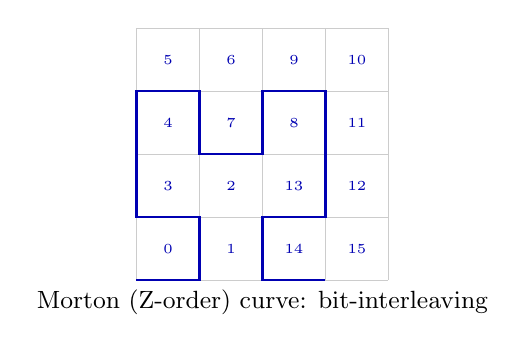
\begin{tikzpicture}[scale=0.8]
  \draw[gray!40,thin] (0,0) grid (4,4);
  \draw[blue!70!black,thick] (0,0)--(1,0)--(1,1)--(0,1)--(0,2)--(0,3)--(1,3)--(1,2)--(2,2)--(2,3)--(3,3)--(3,2)--(3,1)--(2,1)--(2,0)--(3,0);
  \foreach \x/\y/\c in {0/0/0, 1/0/1, 1/1/2, 0/1/3, 0/2/4, 0/3/5, 1/3/6, 1/2/7, 2/2/8, 2/3/9, 3/3/10, 3/2/11, 3/1/12, 2/1/13, 2/0/14, 3/0/15} {
    \node[font=\tiny,blue!70!black] at (\x+0.5,\y+0.5) {\c};
  }
  \node[below,font=\small] at (2,0) {Morton (Z-order) curve: bit-interleaving};
\end{tikzpicture}
\caption{Morton curve: the Z-shaped traversal is obtained by interleaving the binary representations of $x$ and $y$.}
\label{fig:morton_curve}
\end{figure}


\subsection{Pseudocode}
\begin{algorithm}
\caption{Morton Code: Coordinates to Index}\label{alg:xy_to_morton}
\begin{algorithmic}
\Function{XYtoMorton}{x, y}
    \State $morton\_code \gets 0$
    \Comment{Process bits one by one}
    \For{$i \text{ in range}(MAX\_BITS)$}
        \Comment{Extract $i$-th bit from $x$ and $y$}
        \State $bit\_x \gets (x \gg i) \ \& \ 1$
        \State $bit\_y \gets (y \gg i) \ \& \ 1$

        \Comment{Interleave bits: $y_i$ at position $2i+1$, $x_i$ at position $2i$}
        \State $morton\_code \gets morton\_code \mid (bit\_x \ll (2 \cdot i))$
        \State $morton\_code \gets morton\_code \mid (bit\_y \ll (2 \cdot i + 1))$
    \EndFor

    \Return $morton\_code$
\EndFunction

\Statex

\Comment{Faster version using bit manipulation magic (for 16-bit $x$, $y$)}
\Function{InterleaveBits}{x}
    \State $x \gets (x \mid (x \ll 8)) \ \& \ \texttt{0x00FF00FF}$
    \State $x \gets (x \mid (x \ll 4)) \ \& \ \texttt{0x0F0F0F0F}$
    \State $x \gets (x \mid (x \ll 2)) \ \& \ \texttt{0x33333333}$
    \State $x \gets (x \mid (x \ll 1)) \ \& \ \texttt{0x55555555}$
    \Return $x$
\EndFunction
\end{algorithmic}
\end{algorithm}
\Cref{alg:xy_to_morton} shows both the straightforward bit-by-bit interleaving and the optimized ``bit manipulation magic'' version that performs the interleave in $O(1)$ constant time using only shifts and masks~\cite{morton1966}.

\subsection{Parameter Selection}
\begin{itemize}
    \item \textbf{Bit Depth}: The number of bits used for each coordinate (e.g., 16 bits for a $2^{16} \times 2^{16}$ grid).
    \item \textbf{Interleaving Order}: Conventionally $y$ bits are placed in higher positions, but $x$-first is also used.
\end{itemize}

\subsection{Complexity}
\begin{itemize}
    \item \textbf{Transformation}: $O(1)$ for fixed-size integers using bit manipulation (or $O(n)$ where $n$ is bits).
    \item \textbf{Space}: $O(1)$ auxiliary space.
\end{itemize}

\subsection{Usages}
\begin{itemize}
    \item \textbf{Quadtrees/Octrees}: Morton codes can be used to uniquely represent nodes in a linear quadtree/octree, making them extremely fast to navigate~\cite{samet1984}.
    \item \textbf{Texture Mapping}: Storing textures in Morton order (often called ``swizzling'') significantly improves GPU texture cache hit rates by ensuring local pixels are stored close together in memory.
    \item \textbf{Spatial Databases}: Efficient range queries and nearest neighbor searches.
    \item \textbf{Video Compression}: Partitioning macroblocks in a locality-preserving order.
    \item \textbf{GPGPU Optimization}: Ordering parallel threads to match memory access patterns.
\end{itemize}

\subsection{Testing Methods and Edge Cases}
\begin{itemize}
    \item \textbf{Invertibility}: Ensure bit-interleaving can be reversed (de-interleaving) to recover the original $(x, y)$ (\cref{thm:morton_unique}).
    \item \textbf{Boundary Points}: Test the mapping at $(0,0)$ and the maximum possible coordinate (e.g., $(2^{16}-1, 2^{16}-1)$).
    \item \textbf{Adjacency}: Note that Z-order has ``jumps'' where sequential points on the curve are geographically distant. Verify that these occur only at specific power-of-two boundaries.
    \item \textbf{High Dimensions}: Test that the code works correctly for 3D $(x, y, z)$ coordinates.
\end{itemize}

\subsection{References}
\begin{itemize}
    \item Morton, G. M. (1966). ``A computer-oriented geodetic data base and a new technique in file sequencing''. IBM Technical Report.
    \item Samet, H. (1984). ``The Quadtree and Related Hierarchical Data Structures''. ACM Computing Surveys.
    \item Wikipedia: Z-order curve
\end{itemize}


\section{Peano Curve}
\label{sec:peano_curve}

\subsection{Overview}
The \index{Peano curve}Peano curve is the first known example of a \index{space-filling curve}space-filling curve, discovered by Giuseppe Peano in 1890~\cite{peano1890}. It is a continuous mapping from a 1D unit interval to a 2D unit square. Unlike the Hilbert curve, which is based on a $2 \times 2$ subdivision, the Peano curve is based on a $3 \times 3$ subdivision. It is an important foundational structure in mathematical analysis and fractal geometry~\cite{sagan1994}.

\subsection{Definitions}
\begin{definition}[Space-Filling Curve (Peano)]\label{def:peano_space_filling}
A continuous function $f \colon [0,1] \to [0,1]^2$ whose image is all of $[0,1]^2$. The Peano curve was the first such function to be constructed, answering a question posed by Cantor about whether a continuous bijection between $[0,1]$ and $[0,1]^2$ exists~\cite{peano1890}.
\end{definition}

\begin{definition}[Order ($n$) of the Peano Curve]\label{def:peano_order}
The number of recursive subdivisions. An order-$n$ Peano curve covers a grid of $3^n \times 3^n$ cells, visiting all $9^n$ cells exactly once.
\end{definition}

\begin{definition}[Locality of the Peano Curve]\label{def:peano_locality}
The property of mapping nearby 1D points to nearby 2D points. The Peano curve preserves locality, but with a different structure than the Hilbert curve due to its ternary subdivision~\cite{sagan1994}.
\end{definition}

\subsection{Theory}
The Peano curve is constructed recursively using a $3 \times 3$ grid~\cite{sagan1994}.
\begin{enumerate}
    \item For order $n=1$, the space is divided into 9 squares.
    \item The curve visits these squares in an S-like pattern, ensuring that it enters and exits each square in a way that allows for continuous connection between neighbors.
    \item Each of the 9 squares is then recursively replaced by a smaller $3 \times 3$ Peano curve. Some of these sub-curves must be reflected or rotated to maintain the overall continuity.
\end{enumerate}

Mathematically, the Peano curve is defined by a base-3 representation of coordinates. Interleaving these base-3 digits (trits) provides the 1D index, though the digits must be flipped for certain sub-quadrants to preserve the curve's continuity.

\begin{theorem}[Peano Curve is Continuous and Surjective]\label{thm:peano_surjective}
The Peano curve $f \colon [0,1] \to [0,1]^2$ is a continuous surjection: for every $(x, y) \in [0,1]^2$, there exists $t \in [0,1]$ such that $f(t) = (x, y)$. However, $f$ is not injective: there exist points in $[0,1]^2$ with multiple pre-images.
\end{theorem}

\begin{proof}
Continuity follows from the uniform convergence of the sequence of piecewise-linear approximations $f_n$. At order $n$, the curve visits all $9^n$ cells in the $3^n \times 3^n$ grid, and consecutive cells share an edge. The maximum distance between $f_n(t)$ and $f_{n+1}(t)$ is $O(3^{-n})$, so $\{f_n\}$ converges uniformly. The uniform limit of continuous functions is continuous. Surjectivity follows because every cell in the grid is visited at every order, so every point in $[0,1]^2$ is a limit of visited cells. Non-injectivity arises because the curve must ``double back'' at certain junction points to maintain continuity~\cite{peano1890,sagan1994}.
\end{proof}

\begin{example}[Peano Curve of Order 1]\label{ex:peano_order1}
An order-1 Peano curve visits all $9$ cells in a $3 \times 3$ grid. A standard traversal in S-pattern order (with appropriate reflections) visits:
\[
(0,0) \to (1,0) \to (2,0) \to (2,1) \to (1,1) \to (0,1) \to
\]
\[
(0,2) \to (1,2) \to (2,2)
\]
This forms a backward-S shape. For order 2, each of these 9 cells is replaced by a $3 \times 3$ sub-grid with appropriate reflections to maintain continuity at the junctions.
\end{example}

\subsection{Pseudocode}
\begin{algorithm}
\caption{Peano Curve: Coordinates to Index}\label{alg:peano_index}
\begin{algorithmic}
\Function{PeanoIndex}{n, x, y}
    \Comment{Mapping coordinates $(x, y)$ to a 1D index}
    \Comment{Based on base-3 representation}
    \State $idx \gets 0$
    \For{$i \text{ in range}(n-1, -1, -1)$}
        \State $trit\_x \gets \lfloor x / 3^i \rfloor \bmod 3$
        \State $trit\_y \gets \lfloor y / 3^i \rfloor \bmod 3$

        \Comment{Handle reflections for even-numbered segments}
        \If{$x\_is\_reversed$}
            \State $trit\_x \gets 2 - trit\_x$
        \EndIf
        \If{$y\_is\_reversed$}
            \State $trit\_y \gets 2 - trit\_y$
        \EndIf

        \Comment{Segment index (0--8)}
        \State $segment \gets trit\_y \cdot 3 + trit\_x$
        \State $idx \gets idx \cdot 9 + segment$

        \Comment{Update reflection state for next level}
        \State \text{UpdateReflectionState}(trit\_x, trit\_y)
    \EndFor

    \Return $idx$
\EndFunction
\end{algorithmic}
\end{algorithm}

\subsection{Parameter Selection}
\begin{itemize}
    \item \textbf{Order ($n$)}: Determines the resolution of the grid ($3^n \times 3^n$).
    \item \textbf{Grid Size}: Must be a power of 3.
\end{itemize}

\subsection{Complexity}
\begin{itemize}
    \item \textbf{Transformation}: $O(n)$ base-3 digit operations.
    \item \textbf{Space}: $O(1)$ auxiliary space.
\end{itemize}

\subsection{Usages}
\begin{itemize}
    \item \textbf{Theoretical Analysis}: A fundamental counter-example in topology and real analysis (showing a continuous mapping from 1D to 2D)~\cite{peano1890}.
    \item \textbf{Image Processing}: Scanning images in a way that respects local structures, similar to Hilbert scans.
    \item \textbf{Data Organization}: Multidimensional indexing (though base-2 curves like Hilbert and Morton are much more common in digital hardware).
    \item \textbf{Fractal Design}: Used in generative art and architectural patterns.
\end{itemize}

\subsection{Testing Methods and Edge Cases}
\begin{itemize}
    \item \textbf{Continuity}: Verify that for any index $i$, the Euclidean distance between \texttt{Peano(i)} and \texttt{Peano(i+1)} is exactly 1 unit in the grid.
    \item \textbf{Full Coverage}: Verify that every $(x, y)$ coordinate in a $3^n \times 3^n$ grid is mapped to a unique index $0 \dots 9^n - 1$.
    \item \textbf{Boundary Cases}: Test coordinates $(0,0)$ and the maximum coordinate $(3^n-1, 3^n-1)$.
    \item \textbf{Reflections}: Carefully test the ``flipping'' logic in the S-pattern to ensure the curve doesn't have breaks.
\end{itemize}

\subsection{References}
\begin{itemize}
    \item Peano, G. (1890). ``Sur une courbe, qui remplit toute une aire plaine''. Mathematische Annalen.
    \item Sagan, H. (1994). ``Space-Filling Curves''. Universitext.
    \item Wikipedia: Peano curve
\end{itemize}


\section{Zigzag Curve}
\label{sec:zigzag_curve}

\subsection{Overview}
The \index{zigzag curve}zigzag curve (or \index{snake scan}snake scan) is a simple space-filling curve that visits every cell in a 2D grid in a back-and-forth pattern. Unlike Hilbert or Morton curves, it does not have fractal properties and is not designed for recursive locality preservation. Instead, it is highly efficient for sequential data access in rectangular arrays and is a common technique in image and video compression~\cite{pennebaker1992}.

\subsection{Definitions}
\begin{definition}[Zigzag Scan]\label{def:zigzag_scan}
A path that traverses a grid row-by-row, alternating the direction of traversal for each row. Even-indexed rows are traversed left-to-right, and odd-indexed rows are traversed right-to-left.
\end{definition}

\begin{definition}[Locality of Zigzag Scan]\label{def:zigzag_locality}
Sequential points on a zigzag curve are geographically close within a row, but there are large jumps when moving between rows. The horizontal locality is perfect (adjacent indices map to adjacent cells), but vertical locality is poor compared to fractal curves.
\end{definition}

\begin{definition}[Raster Scan]\label{def:raster_scan}
A similar scan that always goes in the same direction (e.g., left-to-right). Zigzag is preferred in some cases because it maintains some horizontal locality at the row transitions, avoiding the large horizontal jumps that a raster scan has at each row boundary.
\end{definition}

\subsection{Theory}
The zigzag scan is constructed by iterating through the grid row by row.
\begin{itemize}
    \item For \textbf{even-indexed rows} (0, 2, $\ldots$), the curve moves from left to right.
    \item For \textbf{odd-indexed rows} (1, 3, $\ldots$), the curve moves from right to left.
\end{itemize}

In image compression (like JPEG), a more specific \textbf{diagonal zigzag scan} is used. This scan traverses an $8 \times 8$ block of frequency coefficients in order of increasing frequency. This ensures that the low-frequency coefficients (which carry most of the image information) are grouped together, making them easier to compress~\cite{pennebaker1992}.

\begin{theorem}[Zigzag Scan Covers All Cells]\label{thm:zigzag_complete}
For a $W \times H$ grid, the snake scan produces a path of length $W \cdot H$ that visits every cell $(x, y)$ with $0 \le x < W$ and $0 \le y < H$ exactly once. Consecutive cells in the path are always Manhattan neighbors.
\end{theorem}

\begin{proof}
The scan processes $H$ rows, each containing $W$ cells. For each row $y$, the cells are enumerated in order: if $y$ is even, the cells $(0,y), (1,y), \ldots, (W-1,y)$ are visited; if $y$ is odd, the cells $(W-1,y), (W-2,y), \ldots, (0,y)$ are visited. Within a row, consecutive cells differ by exactly 1 in the $x$-coordinate. Between rows, the last cell of row $y$ and the first cell of row $y+1$ share the same $x$-coordinate (since row $y+1$ starts from the opposite side), so they are Manhattan neighbors. The total number of cells visited is $H \cdot W$, and since each $(x, y)$ with $0 \le x < W$, $0 \le y < H$ appears in exactly one row, the coverage is complete and without repetition.
\end{proof}

\begin{example}[Snake Scan on a $4 \times 3$ Grid]\label{ex:snake_scan}
A $4 \times 3$ grid traversed by snake scan:
\[
(0,0) \to (1,0) \to (2,0) \to (3,0) \to
(3,1) \to (2,1) \to (1,1) \to (0,1) \to
(0,2) \to (1,2) \to (2,2) \to (3,2)
\]
Row 0 (even): left to right. Row 1 (odd): right to left. Row 2 (even): left to right. All 12 cells are visited exactly once, and consecutive cells are Manhattan neighbors as guaranteed by \cref{thm:zigzag_complete}.
\end{example}

\subsection{Pseudocode}

\subsubsection{Standard Snake Scan}
\begin{algorithm}
\caption{Snake Scan Traversal}\label{alg:snake_scan}
\begin{algorithmic}
\Function{SnakeScan}{width, height}
    \State $path \gets []$
    \For{$y \text{ in range}(height)$}
        \If{$y \bmod 2 = 0$}
            \Comment{Even row: left to right}
            \For{$x \text{ in range}(width)$}
                \State $path.\text{append}((x, y))$
            \EndFor
        \Else
            \Comment{Odd row: right to left}
            \For{$x \text{ in range}(width - 1, -1, -1)$}
                \State $path.\text{append}((x, y))$
            \EndFor
        \EndIf
    \EndFor
    \Return $path$
\EndFunction
\end{algorithmic}
\end{algorithm}

\subsubsection{Diagonal Zigzag (JPEG style)}
\begin{algorithm}
\caption{Diagonal Zigzag Scan (JPEG)}\label{alg:diagonal_zigzag}
\begin{algorithmic}
\Function{DiagonalZigzag}{size}
    \Comment{Scan a square block diagonally}
    \State $path \gets []$
    \For{$s \text{ in range}(2 \cdot size - 1)$}
        \If{$s \bmod 2 = 0$}
            \Comment{Up-right diagonal}
            \For{$y \text{ in range}(size)$}
                \State $x \gets s - y$
                \If{$0 \le x < size$}
                    \State $path.\text{append}((x, y))$
                \EndIf
            \EndFor
        \Else
            \Comment{Down-left diagonal}
            \For{$x \text{ in range}(size)$}
                \State $y \gets s - x$
                \If{$0 \le y < size$}
                    \State $path.\text{append}((x, y))$
                \EndIf
            \EndFor
        \EndIf
    \EndFor
    \Return $path$
\EndFunction
\end{algorithmic}
\end{algorithm}
The diagonal zigzag (\Cref{alg:diagonal_zigzag}) is particularly important in JPEG compression~\cite{pennebaker1992}, where it orders DCT coefficients so that low-frequency entries come first, enabling efficient run-length encoding.

\subsection{Parameter Selection}
\begin{itemize}
    \item \textbf{Direction}: Can be row-major (standard snake) or diagonal (compression).
    \item \textbf{Block Size}: For JPEG, the block size is fixed at $8 \times 8$.
\end{itemize}

\subsection{Complexity}
\begin{itemize}
    \item \textbf{Transformation}: $O(1)$ to compute a coordinate from an index (and vice versa) using modular arithmetic.
    \item \textbf{Space}: $O(1)$ auxiliary space.
\end{itemize}

\subsection{Usages}
\begin{itemize}
    \item \textbf{Image/Video Compression (JPEG, MPEG)}: Ordering DCT coefficients to group low-frequency data, which improves the efficiency of run-length encoding (RLE)~\cite{pennebaker1992}.
    \item \textbf{Display Technology}: Scanning pixels in CRT or LCD screens.
    \item \textbf{Robotics/3D Printing}: Planning the path for a nozzle or sensor to cover a flat area (rasterizing a plane).
    \item \textbf{Sensor Networks}: Ordering data collection from a grid of sensors.
\end{itemize}

\subsection{Testing Methods and Edge Cases}
\begin{itemize}
    \item \textbf{Full Coverage}: Verify that every $(x, y)$ in the grid appears exactly once in the scan.
    \item \textbf{Continuity}: Verify that consecutive points in the path are Manhattan neighbors.
    \item \textbf{Non-Square Grids}: Ensure the algorithm handles $W \ne H$ correctly.
    \item \textbf{Zero/One dimensions}: Test on $1 \times N$ or $N \times 1$ grids.
\end{itemize}

\subsection{References}
\begin{itemize}
    \item Pennebaker, W. B., \& Mitchell, J. L. (1992). ``JPEG: Still Image Data Compression Standard''. Van Nostrand Reinhold.
    \item Wikipedia: Zigzag
\end{itemize}


\section{Spiral Walk}
\label{sec:spiral_walk}

\subsection{Overview}
A \index{spiral walk}spiral walk is a space-filling traversal that starts at a center point and visits cells in a 2D grid in an expanding spiral pattern. Unlike Hilbert or Morton curves, which are recursive and locality-preserving, the spiral walk is intuitive and ensures that the distance from the starting point increases monotonically (on average). It is used for localized searching, image scanning, and data visualization.

\subsection{Definitions}
\begin{definition}[Archimedean Spiral]\label{def:archimedean_spiral}
A continuous curve where the distance from the origin is proportional to the angle: $r = a + b\theta$. The discrete square spiral is an approximation to the Archimedean spiral on an integer grid.
\end{definition}

\begin{definition}[Square Spiral]\label{def:square_spiral}
A discrete version of the spiral restricted to a square grid. It visits cells in layers, where layer $k$ consists of the $8k$ cells forming the perimeter of a $(2k+1) \times (2k+1)$ square centered at the origin.
\end{definition}

\begin{definition}[Radius ($r$) of a Spiral Walk]\label{def:spiral_radius}
The maximum Manhattan or Chebyshev distance from the starting point during the walk. After visiting all cells within radius $r$, the total number of cells visited is $(2r+1)^2$.
\end{definition}

\subsection{Theory}
The square spiral walk is typically performed by moving in layers~\cite{stein1964}.
\begin{enumerate}
    \item \textbf{Layer 0}: The starting cell $(0,0)$.
    \item \textbf{Layer 1}: The 8 neighbors surrounding the center.
    \item \textbf{Layer $k$}: The $8k$ cells that form the perimeter of a $(2k+1) \times (2k+1)$ square.
\end{enumerate}

The walk follows a repeating pattern of directions (e.g., Right, Up, Left, Down) with increasing segment lengths. For example:
\begin{itemize}
    \item Right 1, Up 1
    \item Left 2, Down 2
    \item Right 3, Up 3
    \item Left 4, Down 4
    \item \ldots
\end{itemize}

\begin{theorem}[Spiral Walk Coverage]\label{thm:spiral_coverage}
After completing layer $k$ (i.e., after $N = (2k+1)^2$ steps), the spiral walk has visited every cell $(x, y)$ with $|x| \le k$ and $|y| \le k$. The total number of steps to cover a square of radius $r$ is $(2r+1)^2$.
\end{theorem}

\begin{proof}
Layer $k$ adds the cells on the perimeter of the $(2k+1) \times (2k+1)$ square that are not already covered by layers $0, \ldots, k-1$. The number of cells on this perimeter is $(2k+1)^2 - (2(k-1)+1)^2 = (2k+1)^2 - (2k-1)^2 = 8k$. By induction, after completing layer $k$, the walk has visited all cells within the $(2k+1) \times (2k+1)$ square, totaling $\sum_{j=0}^{k} 8j + 1 = (2k+1)^2$ cells~\cite{stein1964}.
\end{proof}

\begin{example}[First 25 Steps of a Square Spiral]\label{ex:spiral_25}
The first 25 steps of the square spiral (covering a $5 \times 5$ square):
\[
(0,0) \to (1,0) \to (1,1) \to (0,1) \to (-1,1) \to (-1,0) \to (-1,-1) \to (0,-1) \to (1,-1) \to
\]
\[
(2,-1) \to (2,0) \to (2,1) \to (2,2) \to (1,2) \to (0,2) \to (-1,2) \to (-2,2) \to (-2,1) \to
\]
\[
(-2,0) \to (-2,-1) \to (-2,-2) \to (-1,-2) \to (0,-2) \to (1,-2) \to (2,-2)
\]
After $25 = (2 \cdot 2 + 1)^2$ steps, all cells in the $5 \times 5$ square are covered, as guaranteed by \cref{thm:spiral_coverage}.
\end{example}

\subsection{Pseudocode}
\begin{algorithm}
\caption{Square Spiral Walk}\label{alg:spiral_walk}
\begin{algorithmic}
\Function{SpiralWalk}{num\_steps}
    \State $x, y \gets 0, 0$
    \State $path \gets [(x, y)]$

    \Comment{Directions: Right, Up, Left, Down}
    \State $dx \gets [1, 0, -1, 0]$
    \State $dy \gets [0, 1, 0, -1]$

    \State $step\_limit \gets 1$
    \State $direction \gets 0$

    \While{$\text{len}(path) < num\_steps$}
        \Comment{Move in current direction for `step\_limit' steps}
        \For{$\_ \text{ in range}(2)$}
            \Comment{Two directions share the same limit}
            \For{$\_ \text{ in range}(step\_limit)$}
                \If{$\text{len}(path) \ge num\_steps$}
                    \State \textbf{break}
                \EndIf
                \State $x \gets x + dx[direction]$
                \State $y \gets y + dy[direction]$
                \State $path.\text{append}((x, y))$
            \EndFor

            \Comment{Change direction}
            \State $direction \gets (direction + 1) \bmod 4$
        \EndFor

        \Comment{Increase segment length after every two turns}
        \State $step\_limit \gets step\_limit + 1$
    \EndWhile

    \Return $path$
\EndFunction
\end{algorithmic}
\end{algorithm}

\subsection{Parameter Selection}
\begin{itemize}
    \item \textbf{Starting Direction}: Can be any of the four cardinal directions.
    \item \textbf{Orientation}: Clockwise vs.\ Counter-clockwise.
    \item \textbf{Step Size}: Standard is 1 unit, but can be larger for sparse sampling.
\end{itemize}

\subsection{Complexity}
\begin{itemize}
    \item \textbf{Time Complexity}: $O(n)$ where $n$ is the number of steps.
    \item \textbf{Space Complexity}: $O(n)$ to store the path coordinates.
\end{itemize}

\subsection{Usages}
\begin{itemize}
    \item \textbf{Search Algorithms}: Finding the nearest point of interest starting from a query location (e.g., ``nearest gas station'' in a local grid).
    \item \textbf{Computer Vision}: Scanning a local neighborhood around a keypoint or feature.
    \item \textbf{Procedural Generation}: Growing a city or a structure from a central ``seed'' location.
    \item \textbf{Data Visualization}: Arranging objects around a center based on their priority or timestamp (e.g., a ``spiral timeline'').
    \item \textbf{Cryptography}: Permuting bits or pixels in a non-linear but deterministic way.
\end{itemize}

\subsection{Testing Methods and Edge Cases}
\begin{itemize}
    \item \textbf{Full Coverage}: Verify that every $(x, y)$ coordinate within a $k$-layer square is visited exactly once.
    \item \textbf{Monotonicity}: Ensure that for any two sequential points $P_i, P_{i+1}$, their coordinates change by exactly 1 unit.
    \item \textbf{Large Step Count}: Verify the coordinates don't drift or skip cells for $n > 10^6$.
    \item \textbf{Start at Edge}: Handle cases where the spiral is constrained within a bounding box and must stop at the edges.
\end{itemize}

\subsection{References}
\begin{itemize}
    \item Stein, M. L., Ulam, S. M., \& Wells, M. B. (1964). ``A Visual Display of Some Properties of the Distribution of Primes''. The American Mathematical Monthly. (The Ulam Spiral).
    \item Gardner, M. (1971). ``The Extraordinary Properties of the Mathematical Constant Pi''. Scientific American.
    \item Wikipedia: Spiral
\end{itemize}
